%%
%% This is file `sample-sigconf-authordraft.tex',
%% generated with the docstrip utility.
%%
%% The original source files were:
%%
%% samples.dtx  (with options: `all,proceedings,bibtex,authordraft')
%% 
%% IMPORTANT NOTICE:
%% 
%% For the copyright see the source file.
%% 
%% Any modified versions of this file must be renamed
%% with new filenames distinct from sample-sigconf-authordraft.tex.
%% 
%% For distribution of the original source see the terms
%% for copying and modification in the file samples.dtx.
%% 
%% This generated file may be distributed as long as the
%% original source files, as listed above, are part of the
%% same distribution. (The sources need not necessarily be
%% in the same archive or directory.)
%%
%%
%% Commands for TeXCount
%TC:macro \cite [option:text,text]
%TC:macro \citep [option:text,text]
%TC:macro \citet [option:text,text]
%TC:envir table 0 1
%TC:envir table* 0 1
%TC:envir tabular [ignore] word
%TC:envir displaymath 0 word
%TC:envir math 0 word
%TC:envir comment 0 0
%%
%% The first command in your LaTeX source must be the \documentclass
%% command.
%%
%% For submission and review of your manuscript please change the
%% command to \documentclass[manuscript, screen, review]{acmart}.
%%
%% When submitting camera ready or to TAPS, please change the command
%% to \documentclass[sigconf]{acmart} or whichever template is required
%% for your publication.
%%
%%
%\documentclass[acmsmall]{acmart}
\documentclass[sigconf]{acmart}
\usepackage{mathtools}
\usepackage{xspace} 
\usepackage{multirow}
%%
%% \BibTeX command to typeset BibTeX logo in the docs
\AtBeginDocument{%
  \providecommand\BibTeX{{%
    Bib\TeX}}}

%% Rights management information.  This information is sent to you
%% when you complete the rights form.  These commands have SAMPLE
%% values in them; it is your responsibility as an author to replace
%% the commands and values with those provided to you when you
%% complete the rights form.
\setcopyright{acmlicensed}
\copyrightyear{2025}
\acmYear{2025}
\acmJournal{TOG}

%% These commands are for a PROCEEDINGS abstract or paper.
% \acmConference[Conference acronym 'XX]{Make sure to enter the correct
%   conference title from your rights confirmation email}{June 03--05,
%   2025}{Woodstock, NY}
%%
%%  Uncomment \acmBooktitle if the title of the proceedings is different
%%  from ``Proceedings of ...''!
%%
%%\acmBooktitle{Woodstock '18: ACM Symposium on Neural Gaze Detection,
%%  June 03--05, 2018, Woodstock, NY}
%\acmISBN{978-1-4503-XXXX-X/2025/06}


%%
%% Submission ID.
%% Use this when submitting an article to a sponsored event. You'll
%% receive a unique submission ID from the organizers
%% of the event, and this ID should be used as the parameter to this command.
\acmSubmissionID{papers\_353s1}

%%
%% For managing citations, it is recommended to use bibliography
%% files in BibTeX format.
%%
%% You can then either use BibTeX with the ACM-Reference-Format style,
%% or BibLaTeX with the acmnumeric or acmauthoryear sytles, that include
%% support for advanced citation of software artefact from the
%% biblatex-software package, also separately available on CTAN.
%%
%% Look at the sample-*-biblatex.tex files for templates showcasing
%% the biblatex styles.
%%

%%
%% The majority of ACM publications use numbered citations and
%% references.  The command \citestyle{authoryear} switches to the
%% "author year" style.
%%
%% If you are preparing content for an event
%% sponsored by ACM SIGGRAPH, you must use the "author year" style of
%% citations and references.
%% Uncommenting
%% the next command will enable that style.
\citestyle{acmauthoryear}


%%
%% end of the preamble, start of the body of the document source.
\begin{document}
%%
%% The "title" command has an optional parameter,
%% allowing the author to define a "short title" to be used in page headers.
\title{Leaf-alias: fast variance-based importance sampling for real-time ray tracing of dynamic emissive textures}

%%
%% The "author" command and its associated commands are used to define
%% the authors and their affiliations.
%% Of note is the shared affiliation of the first two authors, and the
%% "authornote" and "authornotemark" commands
%% used to denote shared contribution to the research.

\author{Jose Aguerre}
\affiliation{%
  \institution{Universidad de la República}
  \city{Montevideo}
  \country{Uruguay}}
\email{jpaguerre@fing.edu.uy}

\graphicspath{{images/}}
%%
%% By default, the full list of authors will be used in the page
%% headers. Often, this list is too long, and will overlap
%% other information printed in the page headers. This command allows
%% the author to define a more concise list
%% of authors' names for this purpose.
% \renewcommand{\shortauthors}{Trovato et al.}
\newcommand{\FLIP}{\protect\reflectbox{F}LIP\xspace}
%%
%% The abstract is a short summary of the work to be presented in the
%% article.
\begin{abstract}
This is the abstract
\end{abstract}

%%
%% The code below is generated by the tool at http://dl.acm.org/ccs.cfm.
%% Please copy and paste the code instead of the example below.
%%
\begin{CCSXML}
<ccs2012>
   <concept>
       <concept_id>10010147.10010371.10010372.10010376</concept_id>
       <concept_desc>Computing methodologies~Reflectance modeling</concept_desc>
       <concept_significance>500</concept_significance>
       </concept>
 </ccs2012>
\end{CCSXML}

\ccsdesc[500]{Computing methodologies~Reflectance modeling}

%%
%% Keywords. The author(s) should pick words that accurately describe
%% the work being presented. Separate the keywords with commas.
\keywords{These are the keywords}
%% A "teaser" image appears between the author and affiliation
%% information and the body of the document, and typically spans the
%% page.

% \begin{teaserfigure}
%   \centering
%   \begin{tabular}{@{}c@{}c@{}c@{}c@{}}
%     \setlength{\fboxsep}{2pt}  % space between image and border
%     \setlength{\fboxrule}{1pt} % border thickness
%     \includegraphics[width=0.24\textwidth, trim=250 0 250 0, clip]{teaser/horse.png} &
%     \includegraphics[width=0.24\textwidth, trim=250 0 250 0, clip]{teaser/micrograin.png} &
%     \includegraphics[width=0.24\textwidth, trim=250 0 250 0, clip]{teaser/sheen.png} &
%     \includegraphics[width=0.24\textwidth, trim=250 0 250 0, clip]{teaser/rocks.png} \\[0pt]
%     \framebox{\includegraphics[width=0.15\textwidth]{micro_samples/ggx_style.pdf}} &
%     \framebox{\includegraphics[width=0.15\textwidth, trim=0 90 0 90, clip]{micro_samples/3.pdf}} &
%     \framebox{\includegraphics[width=0.15\textwidth, trim=0 0 0 90, clip]{micro_samples/palitos.pdf}} &
%     \framebox{\includegraphics[width=0.15\textwidth]{micro_samples/2.pdf}} \\[0pt]
%     GGX Style heightfield &
%     Ellipsoidal micrograins &
%     Microfibers &
%     Random circle particles \\
%     Specular bounces &
%     Specular bounces & 
%     Glossy bounces &
%     Lambertian bounces
%   \end{tabular}
%   \caption{Microgeometries designed and rendered with our tool.}
%   \label{fig:teaser}
% \end{teaserfigure}

\begin{teaserfigure}
  \centering
  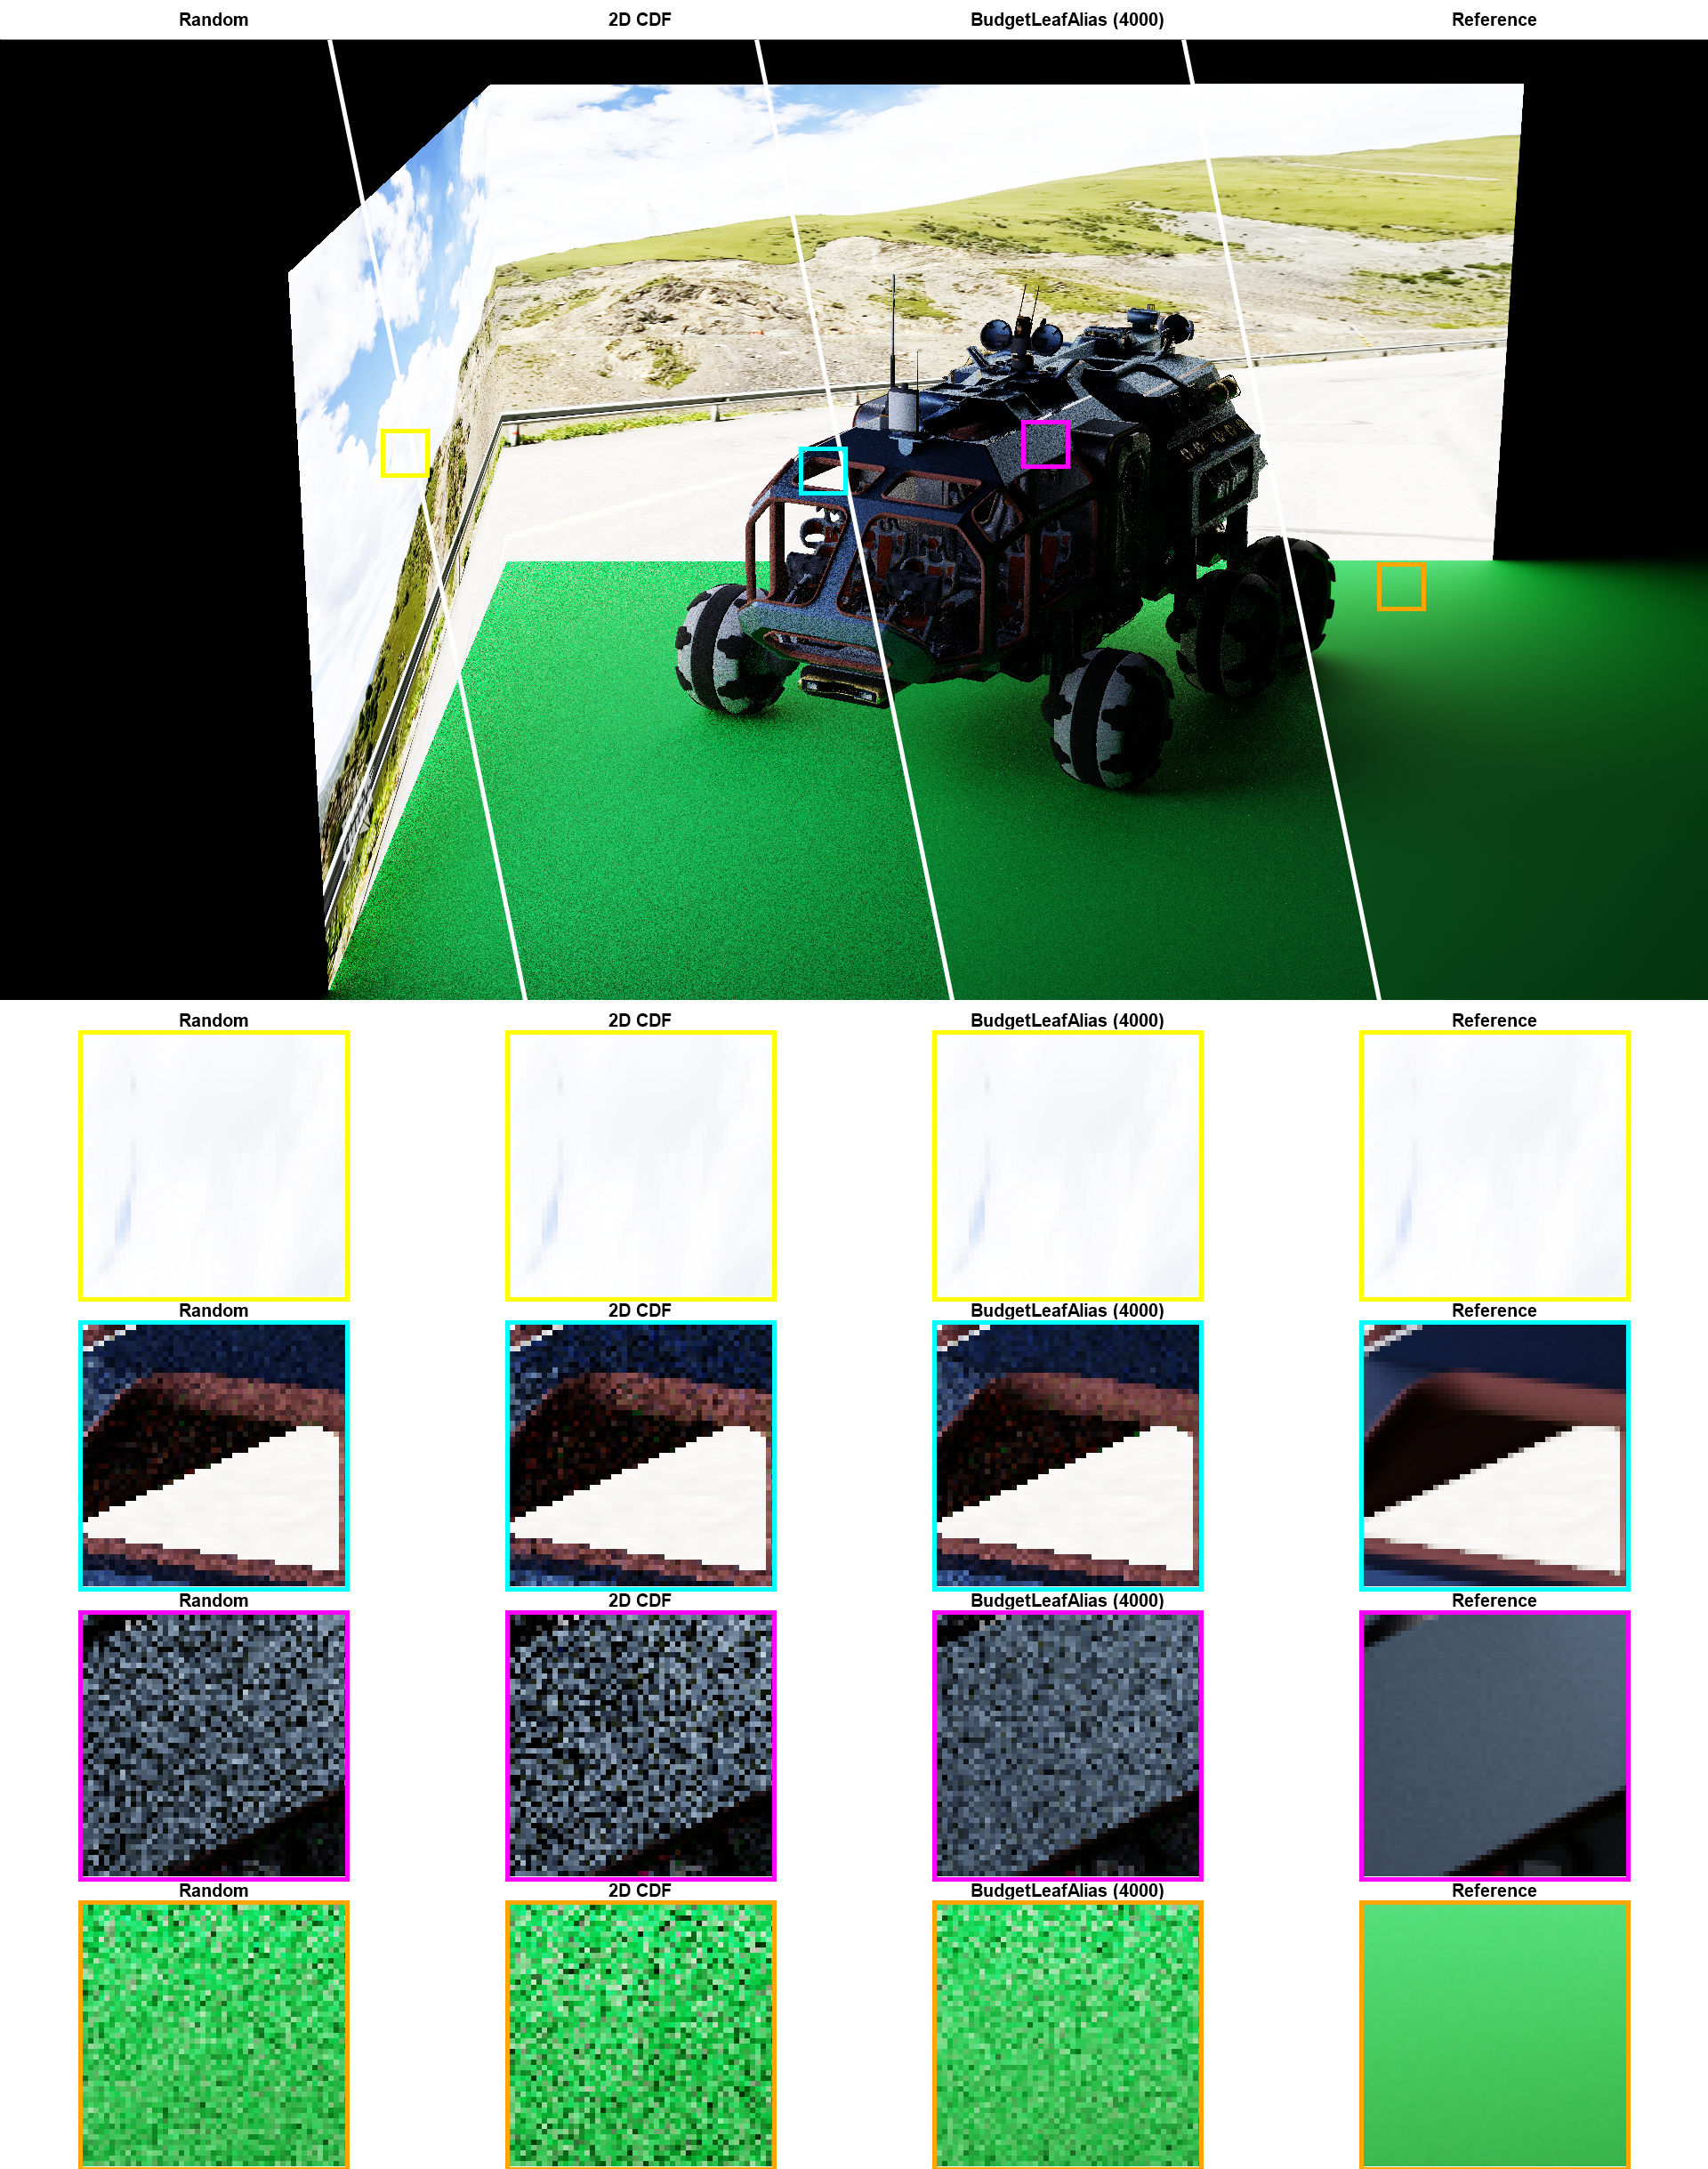
\includegraphics[width=0.5\textwidth]{teaser.png}
  \caption{Teaser caption.}
  \label{fig:teaser}
\end{teaserfigure}



%%
%% This command processes the author and affiliation and title
%% information and builds the first part of the formatted document.
\maketitle

\section{Introduction}
This is the introduction with motivation and background

\section{Previous works}\label{sec:prev}
This is the previous works

\section{Method}\label{sec:method}
This is the method
\subsection{Codec-leaf-alias}
\subsection{Budget-leaf-alias}

\section{Results} \label{sec:results}
These are the results 

\section{Conclusions and future work} \label{sec:conclusions}
These are the conclusions
\bibliographystyle{ACM-Reference-Format}
\bibliography{sample-base}

\end{document}